\documentclass{beamer}
\setbeamertemplate{footline}[page number]
\date{}
\author{}
\institute{}

%%%%%%% Put these names back in the final version 
%\\Aswathy Rajendra Kurup\\Meenu Ajith}
%\institute{Department of Electrical and Computer Engineering\\The University of New Mexico}
\setbeamercovered{transparent}
\usepackage{setspace}
\usepackage{array}
\usepackage[T1]{fontenc}
\usepackage{graphicx}
\usepackage{amsmath}
\usepackage{amsfonts}
\usepackage{amssymb}
\usepackage{makeidx}
\usefonttheme{serif}
\usepackage{multirow}
\usepackage{booktabs} 
\usepackage{rotating}
\usepackage{color}
\usepackage{float}
\usepackage[latin1]{inputenc}
\usepackage[english]{babel}
\usepackage{amsmath}
\usepackage{amsfonts}
\usepackage{eurosym}
\usepackage{rotating}
\usepackage{multicol}
\usepackage{pythonhighlight}
\usepackage[normalem]{ulem}
\newcommand{\ba}{{\bf a}}
\newcommand{\bb}{{\bf b}}
\newcommand{\bc}{{\bf c}}
\newcommand{\bd}{{\bf d}}
\newcommand{\be}{{\bf e}}
\newcommand{\bbf}{{\bf f}}
\newcommand{\bg}{{\bf g}}
\newcommand{\bh}{{\bf h}}
\newcommand{\bi}{{\bf i}}
\newcommand{\bk}{{\bf k}}
\newcommand{\bl}{{\bf l}}
\newcommand{\bm}{{\bf m}}
\newcommand{\bn}{{\bf n}}
\newcommand{\bo}{{\bf o}}
\newcommand{\bp}{{\bf p}}
\newcommand{\bq}{{\bf q}}
\newcommand{\br}{{\bf r}}
\newcommand{\bs}{{\bf s}}
\newcommand{\bt}{{\bf t}}
\newcommand{\bu}{{\bf u}}
\newcommand{\bv}{{\bf v}}
\newcommand{\bw}{{\bf w}}
\newcommand{\bx}{{\bf x}}
\newcommand{\by}{{\bf y}}
\newcommand{\bz}{{\bf z}}

\newcommand{\bA}{{\bf A}}
\newcommand{\bB}{{\bf B}}
\newcommand{\bC}{{\bf C}}
\newcommand{\bE}{{\bf E}}
\newcommand{\bG}{{\bf G}}
\newcommand{\bH}{{\bf H}}
\newcommand{\bI}{{\bf I}}
\newcommand{\bK}{{\bf K}}
\newcommand{\bL}{{\bf L}}
\newcommand{\bM}{{\bf M}}
\newcommand{\bO}{{\bf O}}
\newcommand{\bQ}{{\bf Q}}
\newcommand{\bR}{{\bf R}}
\newcommand{\bS}{{\bf S}}
\newcommand{\bT}{{\bf T}}
\newcommand{\bV}{{\bf V}}
\newcommand{\bW}{{\bf W}}
\newcommand{\bX}{{\bf X}}
\newcommand{\bY}{{\bf Y}}
\newcommand{\bZ}{{\bf Z}}
\newcommand\uptocnt{\stackrel{\mathclap{\normalfont\mbox{c}}}{\propto}}
\newcommand{\bpt}{{\bf pt}}
\newcommand{\bpl}{{\bf pl}}
\newcommand{\bdp}{{\bf dp}}
\newcommand{\btemp}{{\bf temp}}

\newcommand{\bmu}{{\boldsymbol \mu}}
\newcommand{\bSigma}{{\boldsymbol \Sigma}}
\newcommand{\bsigma}{{\boldsymbol \sigma}}
\newcommand{\bvarPhi}{{\boldsymbol \varPhi}}
\newcommand{\bvarphi}{{\boldsymbol \varphi}}
\newcommand{\bPhi}{{\boldsymbol \Phi}}
\newcommand{\bdelta}{{\boldsymbol \delta}}
\newcommand{\bZero}{{\bf 0}}
\newcommand{\bOne}{{\bf 1}}
\newcommand{\balpha}{{\boldsymbol \alpha}}
\newcommand{\bAlpha}{{\boldsymbol A}}
\newcommand{\btheta}{{\boldsymbol \theta}}

\newcommand{\softmax}{\text{softmax}}
\newcommand{\diag}{\text{diag}}
\newcommand{\sinc}{\mathrm{sinc}}
\newcommand{\argmin}{\mathop{\mathrm{argmin}}}
\newcommand{\infl}{\eta}
\newcommand{\Ind}{\mathrm{I}}
\newcommand{\Real}{\mathbb R}
\newcommand{\Intg}{\mathbb Z}
\newcommand{\Complex}{\mathbb C}
\newcommand{\Natural}{\mathbb N}
\newcommand{\Fourier}[1]{\mathcal{F} \{#1\}}
%\newcommand{\ii}{\mathbbm{i}}
\newcommand{\bphi}{\boldsymbol{\mathit{\phi}}}

\newcommand{\hs}{\hspace{2pt}}
\newcommand{\sign}{\text{sign}}
\author{Manel Mart\'inez-Ram\'on\\Meenu Ajith\\Aswathy Rajendra Kurup}

\usetheme{Madrid}
\usecolortheme{beaver}
\usepackage{tikz}
\usetikzlibrary{fit,arrows,calc,positioning}
\usepackage{listings}
\usepackage{xcolor}
\usepackage{emerald} 
\usepackage[T1]{fontenc} 
\usepackage{verbatim}
\usepackage{graphicx}
\usepackage{epsfig}
\usepackage{psfrag}
\usepackage[english]{babel}
\usepackage{listings}
\usepackage{courier}
\usepackage{color}
 \usepackage{vwcol} 
 \usepackage[english]{babel} % To obtain English text with the blindtext package
\usepackage{blindtext}
\definecolor{codegreen}{rgb}{0,0.6,0}
\definecolor{codegray}{rgb}{0.5,0.5,0.5}
\definecolor{codepurple}{rgb}{0.58,0,0.82}
\definecolor{backcolour}{rgb}{0.95,0.95,0.92}

\lstdefinestyle{mystyle}{
  backgroundcolor=\color{backcolour},   commentstyle=\color{codegreen},
  keywordstyle=\color{magenta},
  numberstyle=\tiny\color{codegray},
  stringstyle=\color{codepurple},
  basicstyle=\ttfamily\footnotesize,
  breakatwhitespace=false,         
  breaklines=true,                 
  captionpos=b,                    
  keepspaces=true,                 
  numbers=left,                    
  numbersep=5pt,                  
  showspaces=false,                
  showstringspaces=false,
  showtabs=false,                  
  tabsize=2
}
\lstset{style=mystyle}

%% Stuff for movies

% %\newcommand{\bt}{{\bf t}}
% \newcommand{\br}{{\bf r}}
% \newcommand{\bs}{{\bf s}}
% \newcommand{\by}{{\bf y}}
% \newcommand{\bz}{{\bf z}}
% \newcommand{\bx}{{\bf x}}
% \newcommand{\bw}{{\bf w}}
% \newcommand{\be}{{\bf e}}
% \newcommand{\bbf}{{\bf f}}
% \newcommand{\bb}{{\bf b}}
% \newcommand{\bd}{{\bf d}}
% \newcommand{\bA}{{\bf A}}
% \newcommand{\bB}{{\bf B}}
% \newcommand{\bL}{{\bf L}}
% \newcommand{\bM}{{\bf M}}

% \newcommand{\bC}{{\bf C}}
% \newcommand{\bI}{{\bf I}}
% \newcommand{\bK}{{\bf K}}
% \newcommand{\bk}{{\bf k}}
% \newcommand{\bT}{{\bf T}}
% \newcommand{\bV}{{\bf V}}
% \newcommand{\bW}{{\bf W}}
% \newcommand{\bX}{{\bf X}}
% \newcommand{\bY}{{\bf Y}}
% \newcommand{\bZ}{{\bf Z}}
% \newcommand{\bm}{{\bf m}}
% \newcommand{\bpt}{{\bf pt}}
% \newcommand{\bpl}{{\bf pl}}
% \newcommand{\bdp}{{\bf dp}}
% \newcommand{\btemp}{{\bf temp}}
% \newcommand{\bl}{{\bf l}}
% \newcommand{\bu}{{\bf u}}
% \newcommand{\bmu}{{\boldsymbol \mu}}
% \newcommand{\bSigma}{{\boldsymbol \Sigma}}
% \newcommand{\bLambda}{{\boldsymbol \Lambda}}

% \newcommand{\bsigma}{{\boldsymbol \sigma}}
% \newcommand{\bvarphi}{{\boldsymbol \varPhi}}
% \newcommand{\btheta}{{\boldsymbol \theta}}
% \newcommand{\bZero}{{\bf 0}}
% \newcommand{\balpha}{{\boldsymbol \alpha}}
% \newcommand{\bpi}{{\boldsymbol \pi}}
% \newcommand{\bxi}{{\boldsymbol \xi}}
% \newcommand{\bdelta}{{\boldsymbol \delta}}
\lstset{
	language=Python,
	basicstyle=\footnotesize\ttfamily\color{black},
	commentstyle = \footnotesize\ttfamily\color{red},
	keywordstyle=\footnotesize\ttfamily\color{blue},
	stringstyle=\footnotesize\ttfamily\color{black},
%	columns=fixed,
%	numbers=left,    
	numberstyle=\tiny,
	stepnumber=1,
	numbersep=5pt,
	tabsize=1,
	extendedchars=true,
	breaklines=true,            
	frame=b,         
	showspaces=false,
	showtabs=true,
	xleftmargin=6pt,
	framexleftmargin=6pt,
	framexrightmargin=2pt,
	framexbottommargin=4pt,
	showstringspaces=false      
}

\lstloadlanguages{
         Python
}

%\graphicspath{ {./images/} }  % Figures path - used in graphicx

%\selectcolormodel{cmyk}

\mode<presentation>

\newcommand{\dred}{darkred!90!black}
\newcommand{\written}{\ECFJD\textcolor{cyan!50!white}}
\newcommand{\hlight}{\textcolor{\dred}}
\newcommand{\Ex}{\textcolor{\dred}{Ex. }}

% remove navigation symbols in full screen mode
\setbeamertemplate{navigation symbols}{}  
\setbeamertemplate{blocks}[rounded][shadow=false]
\setbeamercolor{note page}{fg=black}

\setbeamercolor{title}{fg=\dred}
\setbeamercolor{frametitle}{fg=white}
\setbeamercolor{frametitle}{bg=\dred}
\setbeamercolor{structure}{fg=black,bg=white}
\setbeamercolor{background canvas}{bg=white,fg=black}
\setbeamercolor{normal text}{fg=black,bg=white}
\setbeamercolor{item}{fg=red!80!black,bg=white!}
\addtobeamertemplate{block begin}{\setbeamercolor{block title}{fg=white,bg=\dred}
\setbeamercolor{block body}{fg=white,bg=gray}}{}



\title{3. Deep learning tools}
\subtitle{3.4 SciPy}

\addtobeamertemplate{frametitle}{}


\begin{document}

\maketitle

\begin{frame}{Introduction}
\begin{itemize}
    \item Built on top of NumPy.
    \item Optimized to process multidimensional arrays.
    \item A tool to work with
    \begin{itemize}
        \item images and signal processing
        \item large data sets. 
    \end{itemize}
    \item This section contains some examples of the capabilities of the library.  
\end{itemize}
\end{frame}

\begin{frame}[fragile]{Data input and output}
    \begin{itemize}
        \item SciPi is used to work with several data types as .mat, .wav and others, with specific commands for each data type. 
        \item In this example we create, save and load a .mat file, that can be also read in MatLab. 
\begin{lstlisting}
import scipy.io as sio
import numpy as np

arr = np.array([1,2,3,4])  #create an array 
#save the array by the name 'arr_samp'
sio.savemat('sample_data.mat', {'arr_samp': arr}) 
#load the array into the variable from mat file
sample_arr = sio.loadmat('sample_data.mat') 

print(sample_arr['arr_samp'])
\end{lstlisting}
\begin{tiny}
\begin{verbatim}
    [[1 2 3 4]]
\end{verbatim}
\end{tiny}
\end{itemize}
\end{frame}

\begin{frame}[fragile]{Clustering methods}
    \begin{itemize}
        \item Clustering is a procedure that is intended to split a set of data in different points with the purpose of obtaining an interpretation of the data structure. 
        \item A popular rather limited clustering method is K-means, and SciPy has it implemented 
\begin{lstlisting}
from scipy.cluster.vq import kmeans, vq, whiten #importing the packages required for Kmeans clustering
import numpy as np
import matplotlib.pyplot as plt
data1 = np.random.randn(500,2) # Random 2D data 
data2 = np.random.randn(500,2) + np.array([3,3]) 
data = np.vstack((data1,data2)) # stacking the two data 
whit = whiten(data) # whiten the data
[center,_] = kmeans(whit, 2) # Apply Kmeans clustering 
\end{lstlisting}
\end{itemize}
\end{frame}


\begin{frame}[fragile]{Clustering methods}
    \begin{itemize}
        \item This is the representation
\begin{lstlisting}
out = vq(data, center) #assigns labels to data 
plt.scatter(whit[:,0], whit[:,1]) #plot the scatterplots
plt.scatter(center[:,0], center[:,1]) # plot the centroids
plt.show()
\end{lstlisting}
\end{itemize}
\begin{center}
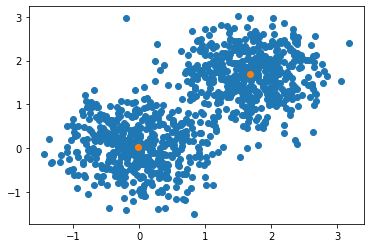
\includegraphics[scale=0.45]{Module 3 (Python tools)/pics/clusters.png}
\end{center}
\end{frame}

\begin{frame}[fragile]{Constants}
\begin{itemize}
    \item \emph{scipy.constants} gives access to many constants. 
    \item They can be used in mathematical expressions. 
\end{itemize}

\begin{lstlisting}
import scipy.constants
from scipy.constants import find

print(find('light')) # find all constants with keyword 'light'
print(scipy.constants.physical_constants['speed of light in vacuum'])
print(scipy.constants.pi) 
\end{lstlisting}
\begin{verbatim}
['speed of light in vacuum']
(299792458.0, 'm s^-1', 0.0)
3.141592653589793
\end{verbatim}

\end{frame}


\begin{frame}[fragile]{Linear algebra}
\begin{itemize}
    \item \emph{scipy.linalg} performs linear algebra operations in Python. 
    \emph Faster than BLAS and LAPACK libraries. 
\end{itemize}

\begin{lstlisting}
from scipy import linalg
import numpy as np

A = np.array([[1,2],[3,2]]) # create a square matrix

print(linalg.det(A))    # compute the determinant of a
print(linalg.inv(A))       # compute the inverse of the matrix
\end{lstlisting}

\begin{verbatim}
-4.0
[[-0.5   0.5 ]
 [ 0.75 -0.25]]
\end{verbatim}
\end{frame}


\begin{frame}[fragile]{Linear algebra}
\begin{lstlisting}
val, vect = linalg.eig(A)  # compute the svd of a
print('\neigenvalues =')
print(val)
print('\neigenvectors =')
print(vect)
b = np.array([2,4])       #  2D vector
print(linalg.solve(a,b))  # Solution of equation Ax=b
\end{lstlisting}

\begin{verbatim}
eigenvalues =
[-1.+0.j  4.+0.j]

eigenvectors =
[[-0.70710678 -0.5547002 ]
 [ 0.70710678 -0.83205029]]

solution of equation Ax=b:  
[1.  0.5]
\end{verbatim}
\end{frame}




\begin{frame}[fragile]{Numeric integrals}
\begin{itemize}
    \item The \emph{integrate} package is used to compute numeric integrals with various methods.
\item Example:
    \begin{equation}\nonumber
        \int_{y=0}^\frac{1}{2}
\int _{x=0}^{1-2y} xydxdy = \frac{1}{96}\approx 0.0104167    \end{equation}
\end{itemize}

\begin{lstlisting}
from scipy import integrate
def f(x, y):
    return x*y
def bounds_y():
    return [0, 0.5]
def bounds_x(y):
    return [0, 1-2*y]

integrate.nquad(f, [bounds_x, bounds_y])
\end{lstlisting}

\begin{verbatim}
(0.010416666666666668, 4.101620128472366e-16)
\end{verbatim}
\end{frame}






\begin{frame}[fragfile]{Optimization}
\begin{itemize}
    \item Minimizing or maximizing a function with constrained and unconstrained minimization problems. \item The package has the most common optimization approaches such as least squares (\emph{least\_squares()}) and curve fitting techniques (\emph{curve\_fit()}).
\end{itemize}
\begin{multicols}{2}
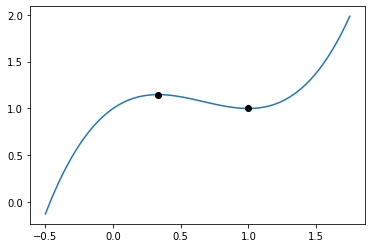
\includegraphics[scale=0.5]{Module 3 (Python tools)/pics/curve.png}

\begin{equation}\nonumber
\begin{split}
    f(x)&=x^3-2x^2+x\\
    f'(x) & = 3x^2-4x+1\\
    x_0&=\frac{1}{3}, ~1
\end{split}
\end{equation}
\end{multicols}
\end{frame}





\begin{frame}[fragile]{}

\begin{lstlisting}
from scipy import optimize
import numpy as np

def func(x):
       return  x**3 -  2*x**2 + x  + 1  # The function

optimize.minimize_scalar(func) # Find the minimum
\end{lstlisting}

\begin{verbatim}
     fun: 1.0
    nfev: 12
     nit: 8
 success: True
       x: 1.0
\end{verbatim}
\end{frame}
\begin{frame}{Other stuff}
\begin{itemize}
    \item The package \emph{interpolate} is also useful. It can interpolate using several methods. 
    \begin{center}
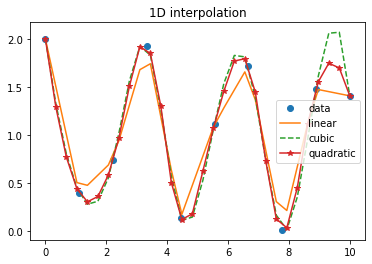
\includegraphics[scale=0.5]{Module 3 (Python tools)/pics/interpolation.png}

\end{center}
    \item The package \emph{scipy.ndimage} can does image processing operations:display, geometric transformations, filtering, edge detection... 
    \item  Library \emph{MISC} is used as a sample to test operations.
\end{itemize}    
\end{frame}

\end{document}

\begin{frame}[fragile]{}
\begin{itemize}
    \item 
\end{itemize}

\begin{lstlisting}
\end{lstlisting}

\begin{verbatim}
\end{verbatim}
\end{frame}
	

